\newcommand{\downloaderTagResultsAucTable}{
    \begin{table}[H]
        \centering
        \begin{tabular}{|p{2,8cm}||P{2,4cm} P{2,4cm} P{2,4cm}|}
            \hline
            Downloader Tag & ALOHA\newline (M/B only) & ALOHA & Proposed\newline Model \\
            \hline
            AUC-ROC & - & 0.967$\pm$0.002 & \textBF{0.983$\pm$0.002} \\
            \hline
        \end{tabular}
        \caption[Downloader Tag prediction task AUC-ROC results]{AUC-ROC (Area Under Curve) of the different models for the \textbf{Downloader Tag} prediction task. Results were aggregated over \textBF{2} training runs with different weight initializations and minibatch orderings. Best results are shown in \textbf{bold}.} \label{tab:downloaderTag_auc}
    \end{table}
}

\newcommand{\downloaderTagResultsAtFprTable}{
    \begin{center}
        \begin{longtable}[c]{|P{3,2cm}||P{1,8cm} P{1,8cm} P{1,8cm} P{1,8cm} P{1,8cm}|}
            \hline
            Downloader Tag & \multicolumn{5}{c|}{{FPR}} \\
            & $10^{-5}$ & $10^{-4}$ & $10^{-3}$ & $10^{-2}$ & $10^{-1}$ \\
            \hline
            \endfirsthead

            \caption*{\raggedright ...continued from previous page} \\
            \hline
            Downloader Tag & \multicolumn{5}{c|}{\textbf{FPR}} \\
            & $10^{-5}$ & $10^{-4}$ & $10^{-3}$ & $10^{-2}$ & $10^{-1}$ \\
            \hline
            \endhead

            \caption*{\raggedleft ...continued on next page} \\
            \endfoot

            \caption[Downloader Tag prediction task results]{Mean and standard deviation results (TPR, Accuracy, Recall, Precision and F1-Score) of the different models for the \textbf{Downloader Tag} prediction task at different \textbf{FPR}s (\textit{False Positive Rates}). Results were aggregated over \textBF{2} training runs with different weight initializations and minibatch orderings. Best results are shown in \textbf{bold}. Under \textbf{TPR} results are also presented the percentage reduction in mean detection error and in ROC curve standard deviation introduced by the \textit{Proposed Model} with respect to both \textit{ALOHA} model and \textit{Joint Embedding}.} \label{tab:downloaderTag_results_at_fpr} \\
            \endlastfoot

            \multicolumn{6}{|c|}{\textbf{TPR}} \\
            \hline
            ALOHA (M/B only) & - & - & - & - & - \\
            ALOHA & \textBF{0.203$\pm$0.060} & 0.306$\pm$0.033 & 0.455$\pm$0.009 & 0.599$\pm$0.018 & 0.877$\pm$0.057 \\
            Proposed Model & 0.196$\pm$0.043 & \textBF{0.489$\pm$0.030} & 0.588$\pm$0.001 & \textBF{0.691$\pm$0.008} & \textBF{0.971$\pm$0.003} \\
            \hline
            Error Reduction wrt\newline ALOHA (M/B only) & - & - & - & - & - \\
            Error Reduction wrt\newline ALOHA & -0.9\% & 26.4\% & 24.4\% & 22.9\% & 76.4\% \\
            \hline
            Std Reduction wrt\newline ALOHA (M/B only) & - & - & - & - & - \\
            Std Reduction wrt\newline ALOHA & 28.3\% & 9.1\% & 88.9\% & 55.6\% & 94.7\% \\
            \hline
            \multicolumn{6}{|c|}{\textbf{Accuracy}} \\
            \hline
            ALOHA (M/B only) & - & - & - & - & - \\
            ALOHA & 0.933$\pm$0.005 & 0.942$\pm$0.003 & 0.954$\pm$0.001 & 0.957$\pm$0.002 & 0.898$\pm$0.005 \\
            Proposed Model & \textBF{0.933$\pm$0.004} & \textBF{0.957$\pm$0.003} & 0.965$\pm$0.000 & \textBF{0.965$\pm$0.001} & \textBF{0.906$\pm$0.000} \\
            \hline
            \multicolumn{6}{|c|}{\textbf{Recall}} \\
            \hline
            ALOHA (M/B only) & - & - & - & - & - \\
            ALOHA & \textBF{0.203$\pm$0.060} & 0.305$\pm$0.033 & 0.455$\pm$0.009 & 0.599$\pm$0.018 & 0.877$\pm$0.057 \\
            Proposed Model & 0.196$\pm$0.043 & \textBF{0.489$\pm$0.030} & 0.588$\pm$0.001 & \textBF{0.691$\pm$0.008} & \textBF{0.971$\pm$0.003} \\
            \hline
            \multicolumn{6}{|c|}{\textbf{Precision}} \\
            \hline
            ALOHA (M/B only) & - & - & - & - & - \\
            ALOHA & \textBF{0.999$\pm$0.000} & 0.996$\pm$0.000 & 0.976$\pm$0.000 & 0.845$\pm$0.004 & 0.444$\pm$0.016 \\
            Proposed Model & \textBF{0.999$\pm$0.000} & \textBF{0.998$\pm$0.000} & \textBF{0.982$\pm$0.000} & \textBF{0.863$\pm$0.001} & \textBF{0.470$\pm$0.001} \\
            \hline
            \multicolumn{6}{|c|}{\textbf{F1 Score}} \\
            \hline
            ALOHA (M/B only) & - & - & - & - & - \\
            ALOHA & \textBF{0.334$\pm$0.083} & 0.467$\pm$0.039 & 0.621$\pm$0.008 & 0.701$\pm$0.014 & 0.589$\pm$0.027 \\
            Proposed Model & 0.326$\pm$0.060 & \textBF{0.656$\pm$0.027} & 0.736$\pm$0.001 & \textBF{0.767$\pm$0.005} & \textBF{0.633$\pm$0.001} \\
            \hline
        \end{longtable}
    \end{center}
}

\newcommand{\downloaderTagResultsSummaryTable}{
    \begin{table}[H]
        \centering
        \begin{tabular}{|P{3,2cm}||P{1,8cm} P{1,8cm} P{1,8cm} P{1,8cm} P{1,8cm}|}
            \hline
            \multicolumn{6}{|c|}{Downloader Tag (at FPR $=1\%$)} \\
            \hline
            Model & TPR & Accuracy & Precision & Recall & F1 score \\
            \hline
            ALOHA (M/B only) & - & - & - & - & - \\
            ALOHA & 0.599$\pm$0.018 & 0.957$\pm$0.002 & 0.845$\pm$0.004 & 0.599$\pm$0.018 & 0.701$\pm$0.014 \\
            Proposed Model & \textBF{0.691$\pm$0.008} & \textBF{0.965$\pm$0.001} & \textBF{0.863$\pm$0.001} & \textBF{0.691$\pm$0.008} & \textBF{0.767$\pm$0.005} \\
            \hline
        \end{tabular}
        \caption[Summary of Downloader Tag prediction task results]{Summary of the mean and standard deviation results of the different models for the \textbf{Downloader Tag} prediction task at \textbf{FPR} $=1\%$. Results were aggregated over \textBF{2} training runs with different weight initializations and minibatch orderings. Best results are shown in \textbf{bold}.} \label{tab:downloaderTag_result_summary}
    \end{table}
}

\newcommand{\downloaderTagRocAlohaMB}{
    \begin{figure}[H]
        \vspace*{-0.5cm}
        \centering
        \includegraphics[width=0.6\textwidth]{./results/downloader_tag_roc_alohaMB.png}
        \vspace*{-0.2cm}
        \caption[Downloader Tag prediction task ALOHA (M/B only) ROC curve]{ROC curve and AUC statistics of \textBF{ALOHA (M/B only)} model for the \textbf{Downloader Tag}. The line represents the \textit{mean} TPR at a given FPR, while the shaded region represents the \textit{standard deviation}. Statistics were computed over \textBF{2} training runs, each with random parameter initialization.}
        \label{fig:downloaderTagRocAlohaMB}
    \end{figure}
}

\newcommand{\downloaderTagRocAloha}{
    \begin{figure}[H]
        \vspace*{-0.5cm}
        \centering
        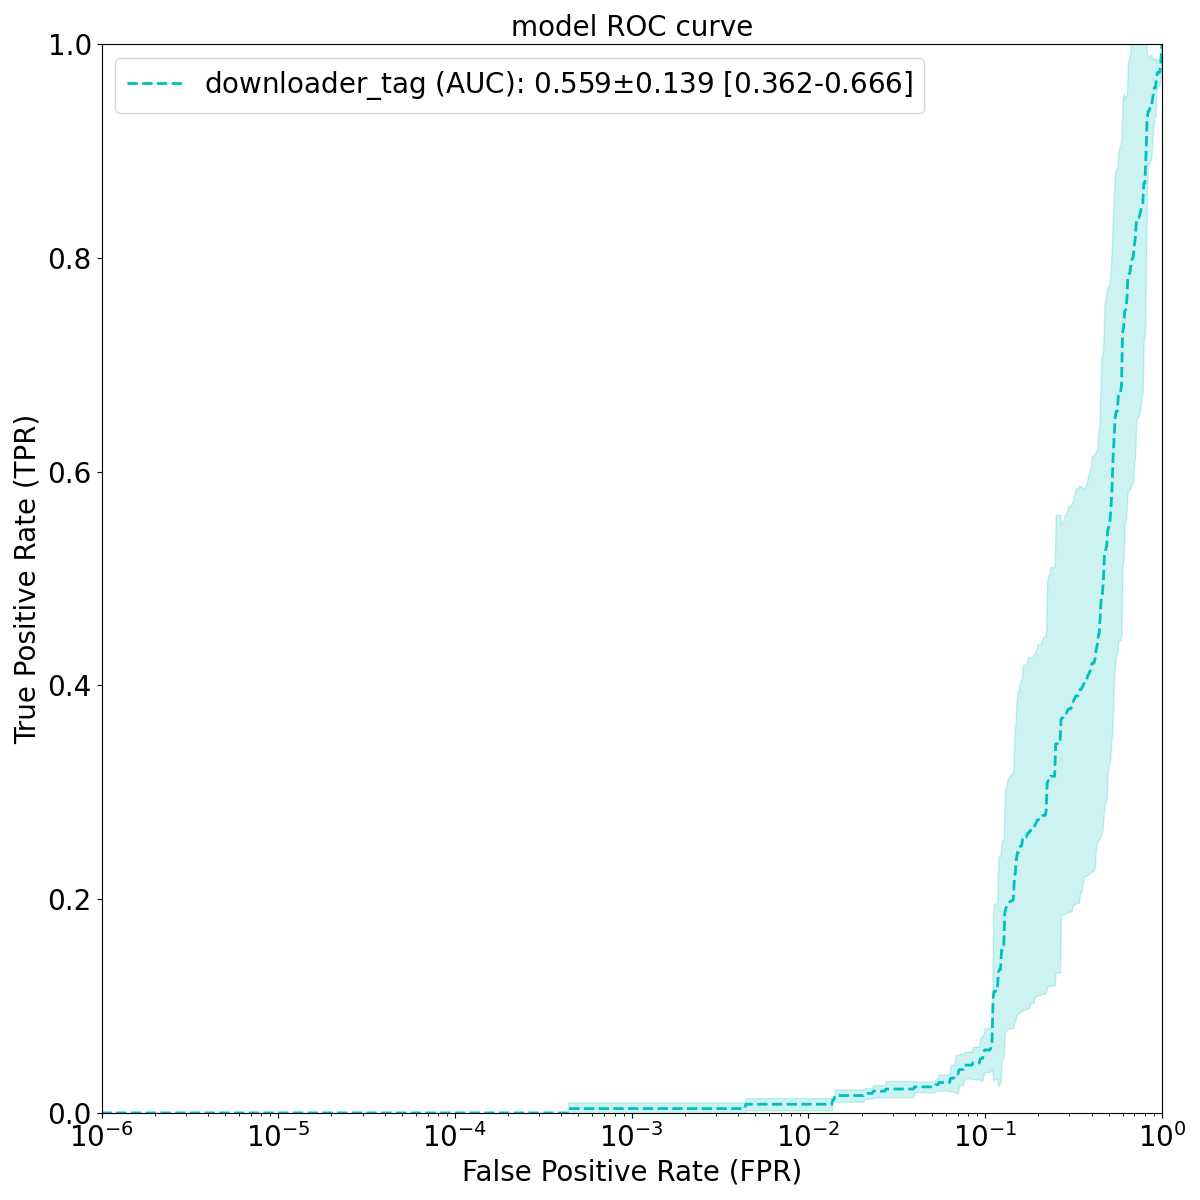
\includegraphics[width=0.6\textwidth]{./results/downloader_tag_roc_aloha.png}
        \vspace*{-0.2cm}
        \caption[Downloader Tag prediction task ALOHA ROC curve]{ROC curve and AUC statistics of \textBF{ALOHA} model for the \textbf{Downloader Tag}. The line represents the \textit{mean} TPR at a given FPR, while the shaded region represents the \textit{standard deviation}. Statistics were computed over \textBF{2} training runs, each with random parameter initialization.}
        \label{fig:downloaderTagRocAloha}
    \end{figure}
}

\newcommand{\downloaderTagRocProposedMethod}{
    \begin{figure}[H]
        \vspace*{-0.5cm}
        \centering
        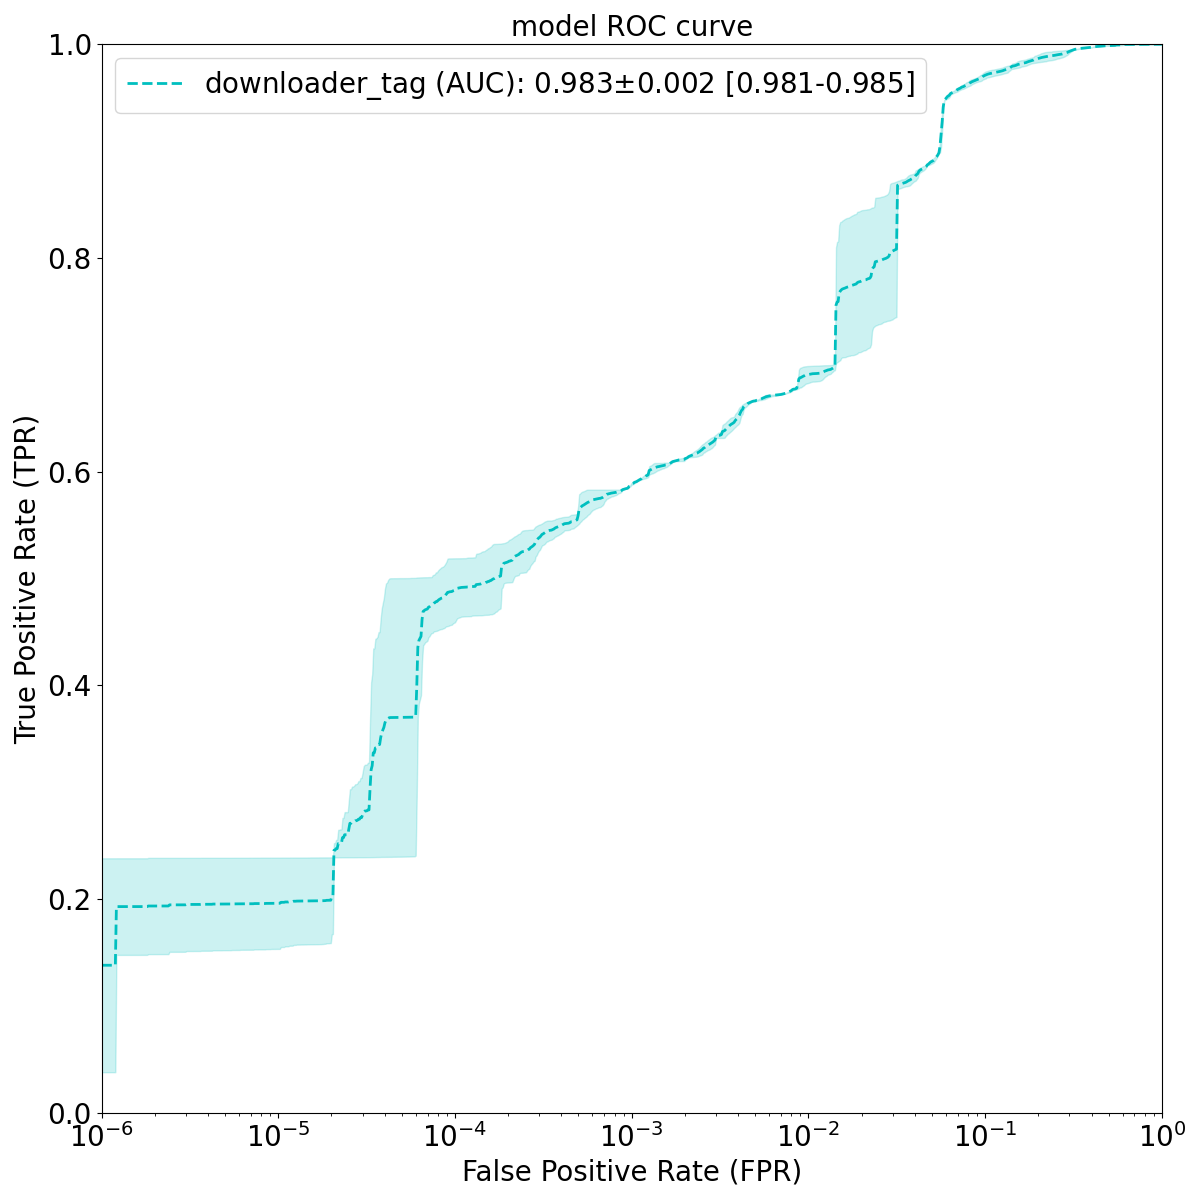
\includegraphics[width=0.6\textwidth]{./results/downloader_tag_roc_proposedModel.png}
        \vspace*{-0.2cm}
        \caption[Downloader Tag prediction task Proposed Model ROC curve]{ROC curve and AUC statistics of \textBF{Proposed Model} for the \textbf{Downloader Tag}. The line represents the \textit{mean} TPR at a given FPR, while the shaded region represents the \textit{standard deviation}. Statistics were computed over \textBF{2} training runs, each with random parameter initialization.}
        \label{fig:downloaderTagRocProposedModel}
    \end{figure}
}
